% status: 2 chapter: Security

\title{Financial Analysis Service}

\author{Rashmi Ray}
\affiliation{%
  \institution{Indiana University}
  \streetaddress{107 S. Indiana Avenue}
  \city{Bloomington}
  \state{Indiana}
  \postcode{43017-6221}
}
\email{rashray@iu.edu}
% The default list of authors is too long for headers}

\renewcommand{\shortauthors}{Rashmi Ray}

\begin{abstract}
  The project analyses how the Kubernetes deployment metdata affects
  performance of a containerized application. The experiment platform will be
  Google Kubernetes Engine. Kubernetes cluster will be setup in a Chameleon
  node to ensure isolated setup. The project will also involve developing a
  Flask REST API for processing stocks data in Python that will provide
  real-time analysis of the stock market data. The performance of the API will
  be compared in both GoogleCloud and local. The stock API will be using
  Python, pyGal, Quandl. The benchmarking process will be registered in the
  project report. 
  
  The project will also discuss the setup process of Google Kubernetes Engine.
   

\end{abstract}

\keywords{hid-sp18-417, Kubernetes, deloyment, performance, GKE, containers}


\maketitle

\section{Introduction}

The area of research for this paper is Kubernetes. In today's age of
containers, it is important for an organization to adopt a container
orchestration and management system, that will also enable seamless
integration and upgrades. Kubernetes is one of the widely popular open source
platform provided for this specific purpose by technology giant Google Inc.
Looking at the high popularity of the tool, it is becoming a buzz word in the
world of cloud computing and containers. The project looks into the ease of
deployment, configuration and performance in Google Kubernetes System. Before
going into the detail of the project outcome, it is important to introduce
several key components of the Kubernetes and GoogleCloud.

\section{Kubernetes}

Kubernetes is an open-source system developed and maintained by Google Inc.
The system provides a container orchestration platform for ease of deployment,
management and scaling of services and resources. The system places containers
automatically based on it resource requirement not compromising availability.
Similarly, it provides seamless management of data volumes and storage system.
It allows updating configurations of the deployment without rebuilding the
image. The system can facilitate public, private or hybrid container
management system based on an organization's requirement.  Kubernetes resource
monitoring system oversees automatic rollout and rollback of the resources in
case of fallbacks.


Kubernetes is also known as K8 or kube. This is originally developed based on
Google's container management system. A Kubernetes can be deployed in a single
host, but it is designed to be benefitted efficiently when used for a cluster
of connected hosts. Use of a cluster of multiple hosts facilitates high
availability.


The primary components of the system are: 

The master node controls the other nodes. Nodes are the hosts in the cluster.
Pod is a group of one or more containers deployed in a node. The Replication
Controller monitors and controls the replicas of the services. A Kubernetes
service is a single unit that has a collection of rules/configuration for
effective deployment of a container. Various metadata such as replicas,
environment, track, port, can be defined in a service configuration.  Kubectl
is the command line configuration tool provided by Kubernetes.

The Figure~\ref{fig:kube-archtecture} explains the Kubernetes architecture.
The master is responsible for managing the deployments, scheduling, exposing
containerized applications.

\begin{figure}[htb]
	\centering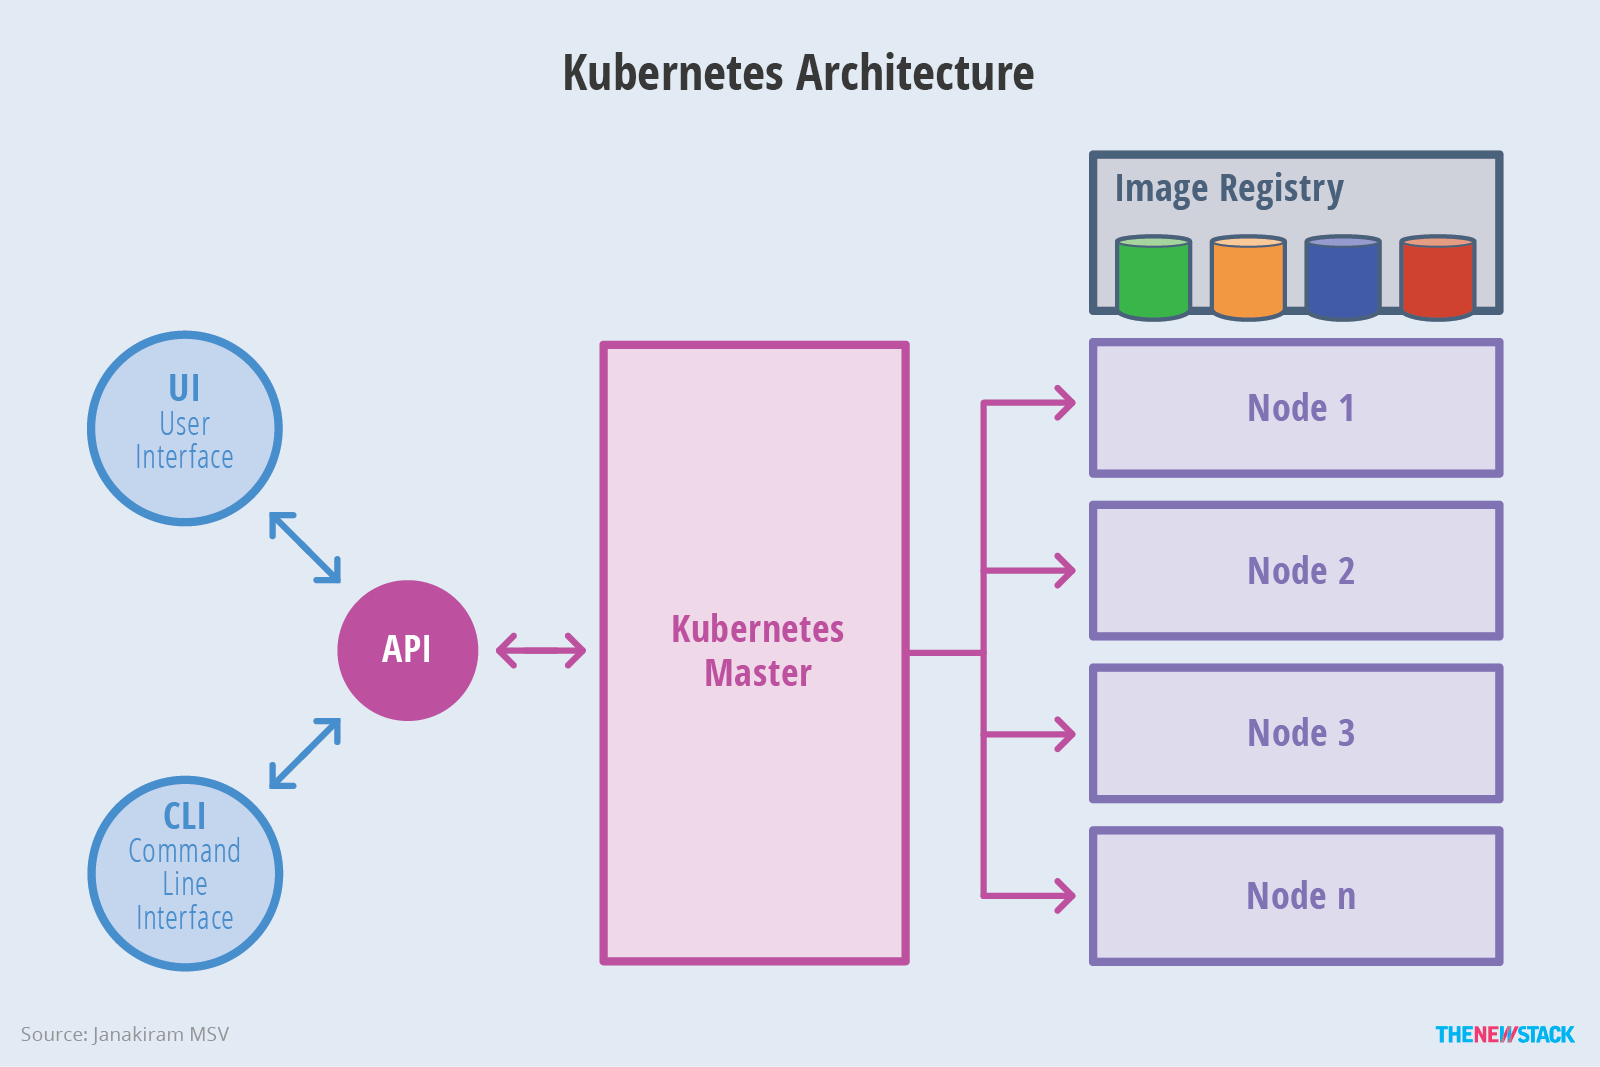
\includegraphics[width=\columnwidth]{images/hid_417_Kubernetes-Architecture.png}
  \caption{Kubernetes Architecture~\cite{hid-sp18-417-kubernetes}}
  \label{fig:kube-archtecture}
\end{figure}


\section{ Google Kubernetes Engine}

Google Kubernetes Engine[GKE] is the tool developed by Google Inc to simplify
the management and orchestration of Kubernetes systems, in Google's public
cloud services. This will help an organization focus more into their ow
product development than worrying about Kubernetes networking, upgrades and
maintenance. As the main focus of the project was Kubernetes, it was vital for
the author to include GKE in the scope of the project.

\subsection{Benefits}

Here are some benefits: With use of GKE, user need not worry about Kubernetes
master. The system ensures that master is always up and running. User need not
worry about underlying networking on what to user e.g. weave, flannel etc.  It
makes access and identity management easier with Google's Identity and
Container Management System[IAM]~\cite{hid-sp18-417-IAM}. Auto scaling is
easier with just simple commands. With Kubernetes' frequent releases it is
important for the system to stay updated always. The upgrade is easier with
gcloud with just a single command rather than the manual overhead of porting
the system step by step.

\subsection{Initial Setup}

The project availed the free tier offer from Google to bring in the setup and
configuration experience for GKE. As of Apr 2018, Google is offering a 300
dollar credit to be used with in 12 months. The free trial has certain
resource usage limitations applied. Please refer to Google's documentation for
details. But the bottom-line was that the limitation was well within the
projects scope to explore the cluster's performance so the author decided to
go ahead with the research.

Here are the key steps involved to get you started with GKE:

\begin{description}

\item[Account Setup] Before you can use GKE, you need to register to google
  cloud. You can use an existing google account. It is required to provide
  credit card information.  Google assures that the card won't be charged
  without your permission.

\item[Shell Setup] GKE provides an option of using google cloud shell [from
  the browser - no installation needed] or local shell [gcloud installation].
  The project kept the local setup in the scope. To set up the environment a
  user must follow the steps listed in Figure~\ref{F:setup}. It includes the
  import of the public key, and installing Google SDK. Aletrnatively, one can
  use the Makefile provided in the project repo to execute the same.

\begin{figure*}[htb]
\begin{footnotesize}
\begin{verbatim}
# Create environment variable for correct distribution
export CLOUD_SDK_REPO='cloud-sdk-$(lsb_release -c -s)'

# Add the Cloud SDK distribution URI as a package source
echo 'deb http://packages.cloud.google.com/apt $CLOUD_SDK_REPO main' | sudo tee -a /etc/apt/sources.list.d/google-cloud-sdk.list

# Import the Google Cloud Platform public key
curl https://packages.cloud.google.com/apt/doc/apt-key.gpg | sudo apt-key add -

# Update the package list and install the Cloud SDK
sudo apt-get update && sudo apt-get install google-cloud-sdk
\end{verbatim}

\end{footnotesize}
\caption{Setup of gcloud SDK}\label{F:setup}
\end{figure*}


\item[Install Kubernetes] Now install Kubernetes:

\begin{verbatim}
sudo apt-get install kubectl
\end{verbatim}

\item[Initiate GoogleCloud] Now GKE is ready to be initiated locally. Before
initiating it is important to know that you will setup the project and compute
zone during the setup. You can setup the compute zone later but it is advised
to set your preference at the beginning to ensure that your requests are
directed in the nearest processing center. [Still to discover more about
zones, but went ahead a selected central-zone-1] 

Now ready to initiate gcloud:
\begin{verbatim}
  gcloud init
\end{verbatim}

\item[Create Cluster] A cluster consists of one master multiple worker
machines. gcloud creates a cluster of three nodes by default. This takes
couple of seconds. Once done it is important to get the credential, so that
containers can be deployed in the cluster. During the project this process
consistently recorded to be more than two
minutes~\cite{hid-sp18-417-cluster-creation-video}.

  \begin{verbatim}
    gcloud container clusters create [CLUSTER_NAME]
  \end{verbatim}
\item[Deployment] A containerized docker image can be deployed to the cluster
using the following:
\begin{verbatim}
  kubectl run [SERVICE_NAME] --image [IMAGE_NAME] 
          --port [port number]
\end{verbatim}
\item [Exposing Service] Exposing a service to a port will enable external
access: [A loadbalancer exposes the service externally.]
\begin{verbatim}
  kubectl expose deployment [SERVICE_NAME] 
        --type 'LoadBalancer'
\end{verbatim}

Once exposed it may take a moment for the service to get exposed. The external
IP can be fetched using the following:

\begin{verbatim}
  kubectl get service [SERVICE_NAME]
\end{verbatim}

\item [External Access] Once the IP is shown, the exposed contained can be
accessed in any web browser.
\begin{verbatim}
  http://[EXTERNAL_IP]:[EXPORTED_PORT]
\end{verbatim}

\item [Cleanup] Finally, here are some useful clean up commands:
\begin{verbatim}
  kubectl delete pod [POD_NAME]
  kubectl delete service [SEVICE_NAME]
  kubectl delete deployment [DEPLOYMENT_NAME]
  gcloud container clusters delete [CLUSTER_NAME]
\end{verbatim}

  Please keep in mind that if a pod is generated through a deployment then to
  remove it the deployment has to be deleted. Deleting the pod will regenerate
  the pod because the replication manager is monitoring the failure and
  handling them.

\end{description}


This Figure~\ref{fig:gcloud-dashboard} shows the GKE dashboard in the current
state. Some of the vital sections are useful to discussed. The current balance
is for the account is shown shown in the top-left corner. In the left menu
option will provide the current state of the account.Identify the active
projects through the project name and ID in the top left block in the content
area. The resources block displays the details of the resources used in the
project. The middle column displays current state of the compute engine and
request/response flow for the containerized APIs. The Google Browser Shell can
be used as an alternative to the local shell.



\begin{figure}[htb]
 \centering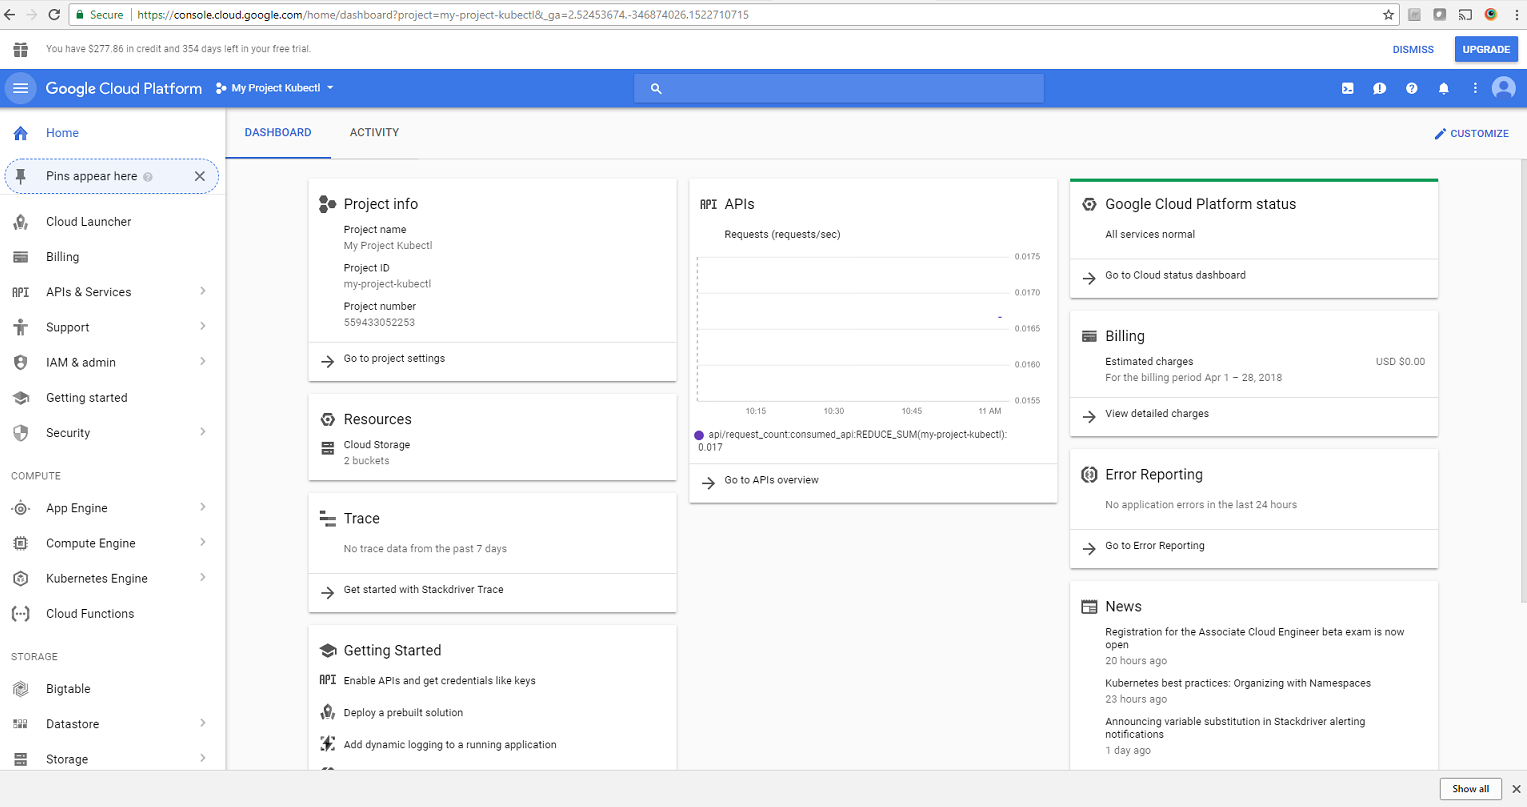
\includegraphics[width=\columnwidth]{images/hid_417_gcloud_browser.png}
 \caption{gcloud Dashboard}\label{fig:gcloud-dashboard}
\end{figure}

 
\section{API in Use}

Before the project is discussed, its important to discuss the following tools
and technologies used in the project. The following subsections also discuss
the necessary installation and code pertaining to the project.


\subsection{Python - API}
Python is a high-level object-oriented programming language. The language is
popular because of its simple readable syntax, minimal required setup and high
availability of large collection of free libraries. The project uses Python
2.7 that is available in the native version of Ubuntu 16.04.

\subsection{Flask - Rest Service}
Flask is a micro framework developed for web development. The framework is
widely popular because its light weight and has minimal dependencies. Flask
was originally written in Python. Some of the key features of Flask are
integrated rest service, secure cookies and unit testing support. The
framework is also compatible with Google App
Engine~\cite{hid-sp18-417-google_appengine}

Flask-RESTful is an extension of Flask that supports quick and easy API
deployments with minimal setup. In order to use the rest service in Python the
Flask module needs to imported. As this project uses Python 2.7, the Flask
compatible version used is 0.10.1 . Here is the basic minimun information
needed to get started with the REST service.

main.py code:

\begin{verbatim}
  from flask import Flask
  app = Flask(__name__)

  @app.route('/')
  def init_func():
        code here
\end{verbatim}

Just install Flask for the installed version of Python.

\begin{verbatim}
  sudo apt-get install python-flask
\end{verbatim}

Here is how to execute the code:
\begin{verbatim}
  python main.py
\end{verbatim}

Here is the sample console output when the Flask server spins up

\begin{verbatim}
  * Running on http://localhost:5000/
\end{verbatim}
A point worth noting here is that Flask server spins up in 5000 port by
default. While exploring exposing the web service on gcloud, the following
command was found inevitable.

\begin{verbatim}
  if __name__ == '__main__':
    app.run(host = '0.0.0.0', debug = False, 
            port=int(os.getenv('PORT', '5000')))
\end{verbatim}

\subsection{Quandl - Realtime Data provider}
Quandl~\cite{hid-sp18-417-Quandl} is a useful Python module that brings in
millions of datasets pertaining economics and finance data. 

Installation:

\begin{verbatim}
  easy_install quandl
\end{verbatim}
The data is available free, but Quandl requires you to register with them in
order to avail critical data. There are still some data available in public
that doesn’t need any registration code. The code can be formatted to receive
data is one of the available formats i.e. json, excel, csv. To retrieve data
from quandl two vital parameters are needed: source code and the ticker code.

The project is using 'WIKI/PRICES' source and ticker is expected to be a
trading code for a desired organization.
\begin{verbatim}
  completeData = qd.get_table('WIKI/PRICES', ticker =
   [companycode])
\end{verbatim}

In the project ticker is set to be query param for the flask REST api.
\begin{verbatim}
  http://localhost:5000/home?code={code}
\end{verbatim}
\subsection{Pygal - Graph Module}
Pygal~\cite{hid-sp18-417-Pygal} is a Python module for interactive plotting.
There other Python modules are available in Python, but Pygal specializes in
SVG~\cite{hid-sp18-417-SVG} graphics.

Installation:

\begin{verbatim}
  easy_install pygal
\end{verbatim}

These graphics being scalable and light weight, they are preferred for
websites. The project chose Pygal for the very specific reason. It collects
real-time data taking in the user entered code in the query prams and renders
the specific a line chart using the respective data collected from Quadl.
\begin{verbatim}
   completeData = qd.get_table('WIKI/PRICES', ticker =
   [companycode])line_chart = pg.Line()
   line_chart.title = 'Stocks Analysis for ' + companycode
   line_chart.add('high', mydata['high'])
   line_chart.add('low',   mydata['low'])
   line_chart.add('close', mydata['close'])
   chart = line_chart.render_data_uri()
\end{verbatim}
\begin{figure}[htb]
	\centering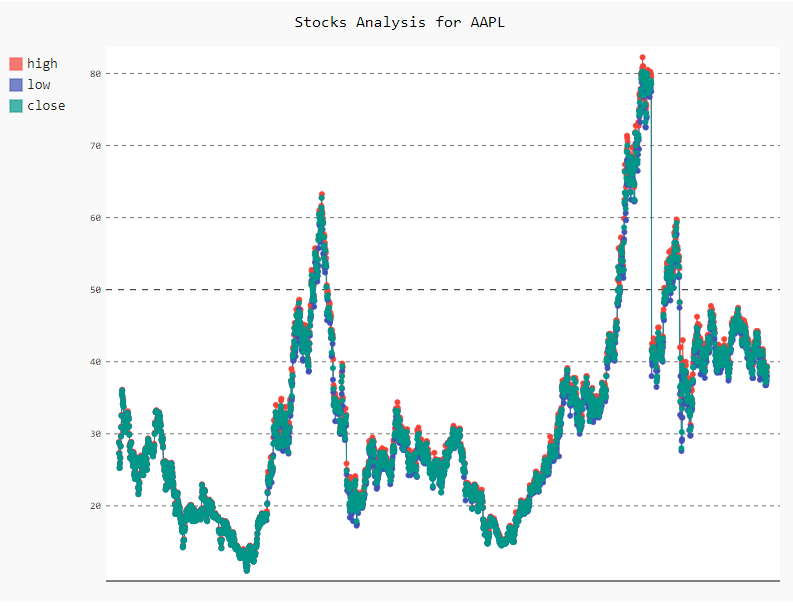
\includegraphics[width=\columnwidth]{images/hid_417_project_graph.png}
  \caption{Project Graph}
  \label{fig:project_graph}
\end{figure}
\subsection{Datetime}

The project uses the Python datetime module to record the data download time
and processing time.
\begin{verbatim}
  Data Load Time: 0:00:03.251368

  Data Processing Time: 0:00:01.612638
\end{verbatim}

\subsection{Docker - Container}
Docker is an opensource tool that enables virtualization at the Operating
System level. The process is also known as containerization. Docker was
primarily developed for Linux system to containerize an application and its
dependencies so that the application can run in any Linux system.

Installation:
\begin{figure*}[htb]
\begin{footnotesize}
\begin{verbatim}
  sudo apt-get update
  sudo apt-get install apt-transport-https ca-certificates curl software-properties-common
  curl -fsSL https://download.docker.com/linux/ubuntu/gpg | sudo apt-key add -
  sudo apt-key fingerprint 0EBFCD88
  sudo add-apt-repository 'deb [arch=amd64] https://download.docker.com/linux/ubuntu $(lsb_release -cs)  stable'
  sudo apt-get update
  sudo apt-get install docker-ce
  sudo apt-get update
\end{verbatim}
\end{footnotesize}
\caption{Docker Installation}\label{F:setup}
\end{figure*}
For the project the stocks microservice is containerized to be deployed in
Kubectl using a Dockerfile~\cite{hid-sp18-417-Dockerfile}.

\subsection{Docker-compose - Container Management}
Docker Compose is a tool used for managing metadata for multi-container
applications. Docker-compose.yml~\cite{hid-sp18-417-docker-compose} was not
mandatory for this project, but was incorporated keeping future improvisations
in mind. 

Installation:

\begin{figure*}[htb]
\begin{verbatim}
  sudo curl -L https://github.com/docker/compose/releases/download/1.18.0/docker-compose-`uname -s`-`uname -m` -o /usr/local/bin/docker-compose
  sudo chmod +x /usr/local/bin/docker-compose
\end{verbatim}
\caption{Docker-compose Installation}
\end{figure*}

\subsection{Makefile}
Makefile is a file that contains instructions to get certain task done. The
project has provided a Makefile that takes care of building a cleaning up the
Docker container. To use this file ensure build-essentials is installed.

Provisioning of Makefile makes the automation process simpler. The project
repo provides two Makefiles. One for gcloud installation and setup, the other
one is for the deployment of the python-flask microservice.
  
\subsection{YAML - Kubernetes Configuration}
It is a good practice to manage Kubernetes deployment through yml files. The
step is not mandatory but desirable for ease of maintenance and Convenience.
Yaml is a markup language that is popularly used for specifying
configurations. If multiple structure are defined in one single file then its
separated by --- . Here is an extract of the yml file used for the project.
Few metadata worth noting is apiversion, kind, replicas, containerPort.
Figure~\ref{F:svc-setup} provides a sample configuration file used for the
project.

\begin{figure}
\begin{footnotesize}  
\begin{verbatim}
apiVersion: extensions/v1beta1
kind: Deployment
metadata:
  name: web-ui
spec:
  replicas: 3
  template:
    metadata:
      labels:
        role: web-ui
    spec:
      containers:
      - name: web-ui
        image: rashray/stocks
        ports:
        - containerPort: 5000
  
\end{verbatim}
\end{footnotesize}
\caption{Deployment Configuration}\label{F:svc-setup}
\end{figure}
\subsection{Chameleon}
Once the required knowledgebase is ready, project was set up in Chameleon
cloud node to ensure that all the required installation and configurations are
registered appropriately for the report.

\subsection{Setup}

Once the Python API was developed it was tested to retrieve the times
recorded. Apple Inc was used for this project. This is because, it has a good
number of records. The Flask server was run locally to check the download and
processing time. The Figure~\ref{fig:project_localhost} depicts the final
webpage.

\begin{figure}[htb]
	\centering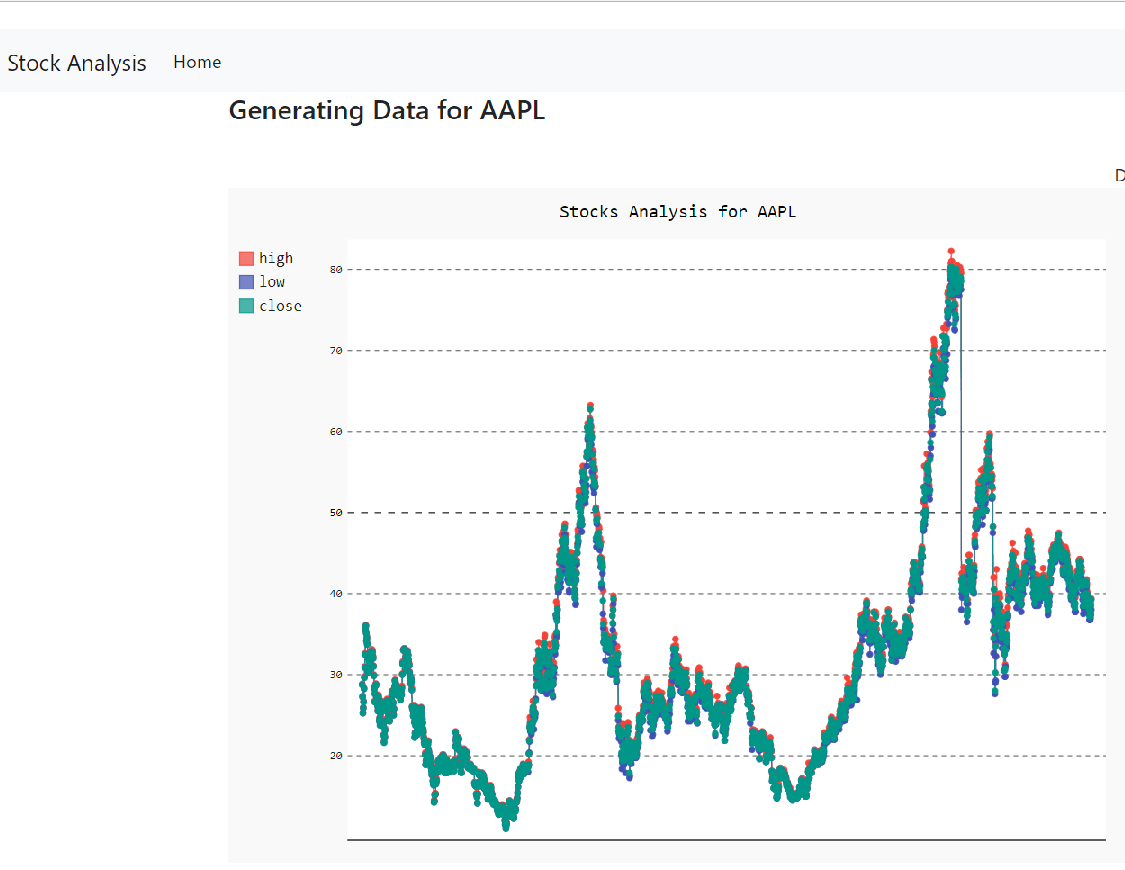
\includegraphics[width=\columnwidth]{images/hid_417_localhost.png}
  \caption{Localhost - REST service}
  \label{fig:project_localhost}
\end{figure}

Now, a Chameleon node was spawn to setup Google Kubernetes Engine. The google
SDK and CLI was installed and configured. 

The Docker image was created using the Makefile:
\begin{verbatim}
 make docker-build
\end{verbatim}
A kubectl cluster was created and it was ensured that the nodes are up and
running.

kubectl get nodes

The web service was deployed.

\begin{verbatim}
  docker-compose up -d

  kubectl apply -f kubernetes/flask-web-ui.yml
\end{verbatim}

Once deployed, it takes around a minute for the external IP to be available.
With the available external IP, User can access the deployed microservice from
anywhere. The default flask-web-ui.yml in the git repo defines 3 replicas.

A short video was recorded to present the overview of the
project~\cite{hid-sp18-417-project_overview}.

Finally once all the required data was collected the deployment and cluster
was cleaned up.

A demonstration of the replication manager and the cleanup process is
  recorded~\cite{hid-sp18-417-google_cleanup} during the project.

\subsection{Performance Analysis}

Now that Good Kubernetes Engine is explored for ease of deployment and
management, it was important to log an analysis. Timestamp was added in the
Makefile to check on the cluster creation time. It was found that both cluster
creation and deletion take on an average 2 minutes. Similar approach was taken
on checking the time taken to expose a web-service to a specific port. It was
concluded that it takes on an average one minute to avail the external IP. 

Depending of the web traffic estimated the number of replication of webservice
is defined so that the fall backs can appropriately addressed. Though
Kubernetes replication manager monitors the resources and pods to ensure that
replications mentioned for a deployment is maintained, it take few seconds for
the restoration to take place in case of fallbacks. The presence of
replications balances the loads and manages fall-backs. Behind the scenes all
the user requests are directed to the master, which in turn directs traffic
appropriately to ensure even distribution. As a part of the benchmarking
process, it was analyzed if the number of service replicas affect performance.


The Python-Flask microservice developed for the stock analysis has two
components one is fetching the stocks data from WIKI and the other is to
process the data in order to render the pygal graph. Python script was added
to log both the download and processing time. Now this timing was compared to
check if a gcloud deployment replicas affect the processing time. The times
were logged initially by running the service locally and then later in the
gcloud cluster. The replicas were changed by changing the respective metdata
in kubectl yml file in API codebase. This is how processing time was logged
for: local-flask server run, containerized microservice with 3, 2 and 1
replica in a gcloud kubernetes cluster. Time in case was recorded five times
and the mean of each set was taken in consideration.


The Figure~\ref{fig:project_deployment} depicts the confiuration change to
deploy the microservice with single replica.

\begin{figure*}[htb]
  \begin{footnotesize}  
  \begin{verbatim}
  cc@kubenode:~/hid-sp18-417/project-code/API/flask$ cat kubernetes/flask-web-ui.yml
---
apiVersion: extensions/v1beta1
kind: Deployment
metadata:
  name: web-ui
spec:
  replicas: 1
  template:
    metadata:
      labels:
        role: web-ui
    spec:
      containers:
      - name: web-ui
        image: rashray/stocks
        ports:
        - containerPort: 5000

---
apiVersion: v1
kind: Service
metadata:
  name: web-ui
  labels:
    role: web-ui-svc
spec:
  ports:
  - port: 5000
    targetPort: 5000
  selector:
    role: web-ui
  type: LoadBalancer
---
cc@kubenode:~/hid-sp18-417/project-code/API/flask$ docker-compose up -d
Creating flask_web-ui_1 ... done
cc@kubenode:~/hid-sp18-417/project-code/API/flask$ kubectl apply -f kubernetes/flask-web-ui.yml
deployment.extensions "web-ui" created
service "web-ui" created
cc@kubenode:~/hid-sp18-417/project-code/API/flask$ kubectl get services
NAME         TYPE           CLUSTER-IP      EXTERNAL-IP   PORT(S)          AGE
kubernetes   ClusterIP      10.35.240.1     <none>        443/TCP          26m
web-ui       LoadBalancer   10.35.247.125   <pending>     5000:32594/TCP   44s
cc@kubenode:~/hid-sp18-417/project-code/API/flask$ kubectl get services
NAME         TYPE           CLUSTER-IP      EXTERNAL-IP     PORT(S)          AGE
kubernetes   ClusterIP      10.35.240.1     <none>          443/TCP          26m
web-ui       LoadBalancer   10.35.247.125   35.232.229.66   5000:32594/TCP   50s
cc@kubenode:~/hid-sp18-417/project-code/API/flask$ kubectl get pods
NAME                      READY     STATUS    RESTARTS   AGE
web-ui-78496b97dc-mgh2w   1/1       Running   0          13m
cc@kubenode:~/hid-sp18-417/project-code/API/flask$
  \end{verbatim}
\end{footnotesize}  

  \caption{gcloud Deployment - 2 replicas}
  \label{fig:project_deployment}
\end{figure*}

Here is the outcome of the excercise in Figure~\ref{tab:performance}:

\begin{table}[htb]
	\centering
  \caption{Downaload and Processing time in different platforms}\label{tab:performance}

	\begin{tabular}{*{3}{c}}
		\toprule
		Environment & Loading Time  &  Processing time \\
		\midrule
		NA & sec: MS & sec: MS \\
		\midrule
		Local hosting & 4:365  & 2.173 \\
		GKE deployment: 3 replicas & 3:834 & 1:525 \\
    GKE deployment: 2 replicas & 3:246 & 1:671 \\
    GKE deployment: 1 replicas & 3:315 & 1:730 \\
		\bottomrule
	\end{tabular}
\end{table}
A visual reprsentation is also provided in Figure~\ref{fig:benchmark_graph}
\begin{figure}[htb]
	\centering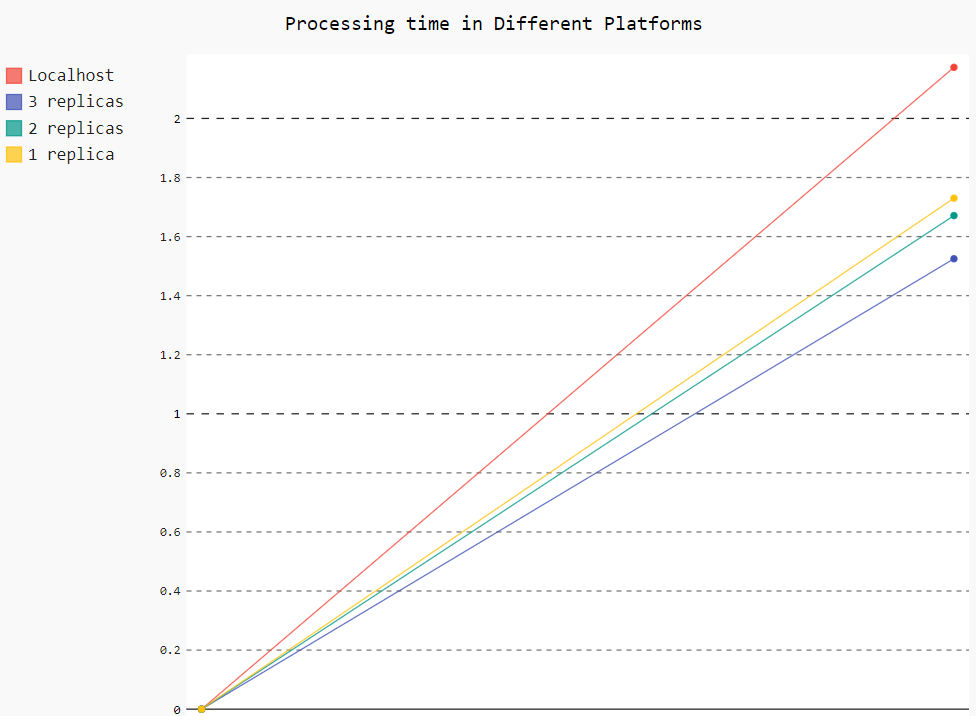
\includegraphics[width=\columnwidth]{images/hid_417_benchmark_graph.png}
  \caption{Graph - Benchmarking Performance Data}
  \label{fig:benchmark_graph}
\end{figure}
With above data the improvement in performance is considerable in the
containerized Kubernetes cluster.
\section{Conclusion}


In the presented work, the developed Flask-Python microservice was
successfully deployed in a GKE cluster. The setup and configuration process
for Google Kubernetes cluster was explained. It was felt that the time
duration for creating and deleting the cluster can be improvised.

It was demonstrated how a replication manager automatically assure that the
deployment configurations are managed in case of fallback. In one of the video
demonstrated how the replication manager monitors and handles fallbacks.

It was also analyzed if the number of replications does affect the performance
of a containerized application. It was found that there is considerable
improvement when locally run service is containerized and deployed in
Kubernetes cluster, but the number of replicas does not affect the performance
much. The automatic monitoring and management of the Kubernetes master makes
the system so efficient.
\begin{acks}
The author would like to thank Dr.\ Gregor von Laszewski for his support and
suggestions in writing this paper.
\end{acks}

\bibliographystyle{ACM-Reference-Format}
\bibliography{report}


